\documentclass[oneside,a4paper,11pt,explicit]{book}
\usepackage[utf8]{inputenc}
\usepackage{icecream}
\usepackage[english]{babel}
\addto\captionsenglish{\renewcommand{\chaptername}{}}
\usepackage[accsupp]{axessibility}  % improves PDF readability for those with disabilities.
\usepackage[colorlinks = true,urlcolor  = blue,linkcolor = blue]{hyperref}
\usepackage{setspace}
\usepackage{listings}
\usepackage[most]{tcolorbox}
\usepackage{minitoc}
\usepackage{multicol}


\renewcommand{\mtifont}{\large\sffamily}
\renewcommand{\mtcfont}{\small\sffamily}
\renewcommand{\mtcSfont}{\small\sffamily}
\renewcommand{\mtcSSfont}{\small\sffamily}
\renewcommand{\mtcSSSfont}{\small\sffamily}
\mtcsetpagenumbers{minitoc}{off} % turn off page numbering in minitocs
\addto{\captionsenglish}{% Making babel aware of special titles
	\renewcommand{\mtctitle}{Quick Links To Sections}
}
\setlength{\fboxrule}{5pt}
\setlength{\fboxsep}{4pt}

\definecolor{IceCreamLeaf}{rgb}{0.4, 0.639215686274, 0.4}
\definecolor{IceCreamOrbit}{rgb}{0.803921568627451, 0.3607843137254902, 0.3607843137254902}

\title{I.C.E.C.R.E.A.M. Tutorials}
\subtitle{\small Observing Earth from Above (Env 329) - Fall 2023  \\
	\small Schmid College of Science and Technology, Chapman University}
\date{\today}

%% DOCUMENT
\setstretch{1.25}
\makeatletter
\begin{document}

\dominitoc

%\tableofcontents

\setcounter{chapter}{7} %Insert (Tutorial Number-1) Here; example for tutorial 4, enter 3

\chapter{Detecting Droughts From Space} %Enter Tutorial Name Here

\vspace{-2em}

\minitoc

\hrule

\vspace{1em}

\begin{tcolorbox}[enhanced,frame style image=blueshade.png,
	opacityback=0.75,opacitybacktitle=0.25,
	colback=blue!5!white,colframe=blue!75!black,title={\Large \textbf{Objectives:}}]
	\large
	\begin{enumerate}
		\item 
	\end{enumerate}
\end{tcolorbox}

\clearpage

%%%%%%%%%%%%%%%%%%%%%%%%%%%%%%%%%% Change Header to Have a Smaller Logo for Remainder of the Document
\fancyhead{}
\fancyhead[C]{\begin{tikzpicture}[overlay, remember picture]
		\fill[Blue2] (current page.north west) rectangle ($(current page.north east)+(0,-1in)$);
		\node[anchor=north west, text=white, font=\Large, minimum size=1in, inner xsep=5mm, align=left] at (current page.north west) {\bf{\MakeUppercase{\@title}}\\\@subtitle};
		\node[anchor=north east, minimum size=1in, inner xsep=5mm] at (current page.north east) {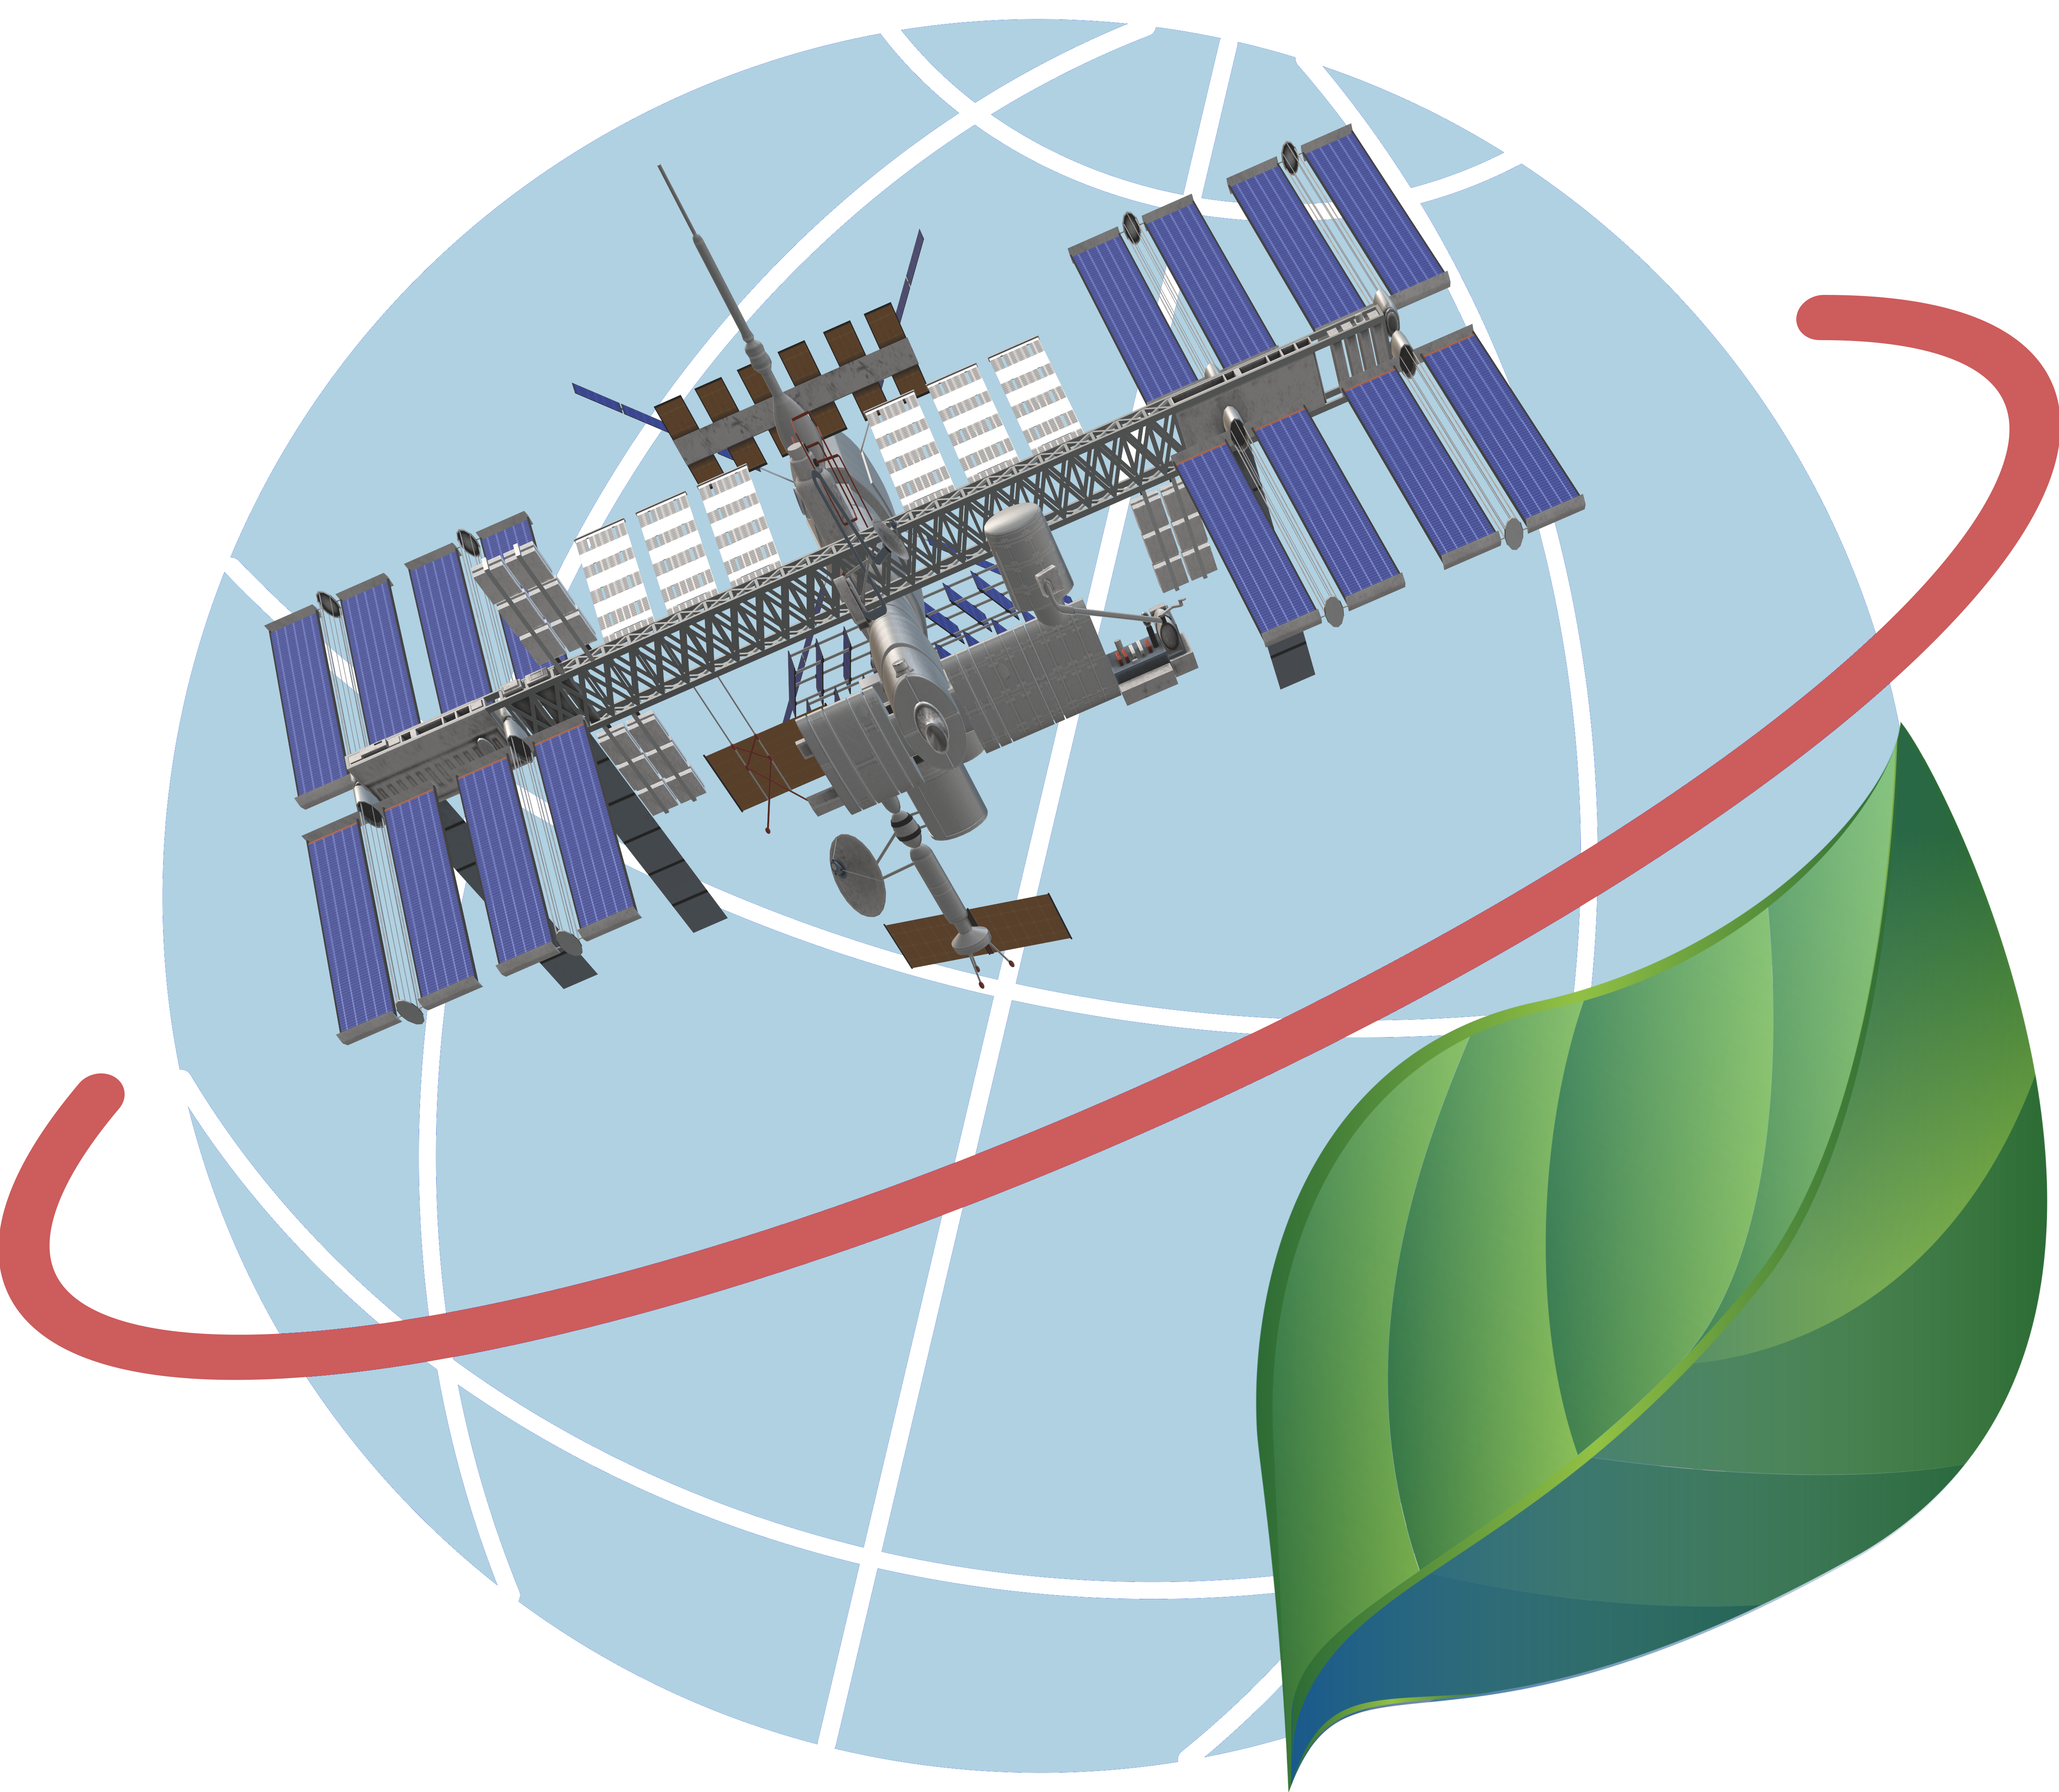
\includegraphics[scale=.125]{ICECREAM_Logo.png}};\end{tikzpicture}}
%%%%%%%%%%%%%%%%%%%%%%%%%%%%%%%%%%

\noindent\fbox{\begin{minipage}{.9665\textwidth}
			
	\vspace{1em}
	\begin{center}
		\textbf{\Large \underline{Motivation For Today's Tutorial : The Global Water Crisis}}
	\end{center}
	
	\addcontentsline{toc}{section}{Motivation : The Global Water Crisis}

	\vspace{1 em}
	
	\centerline{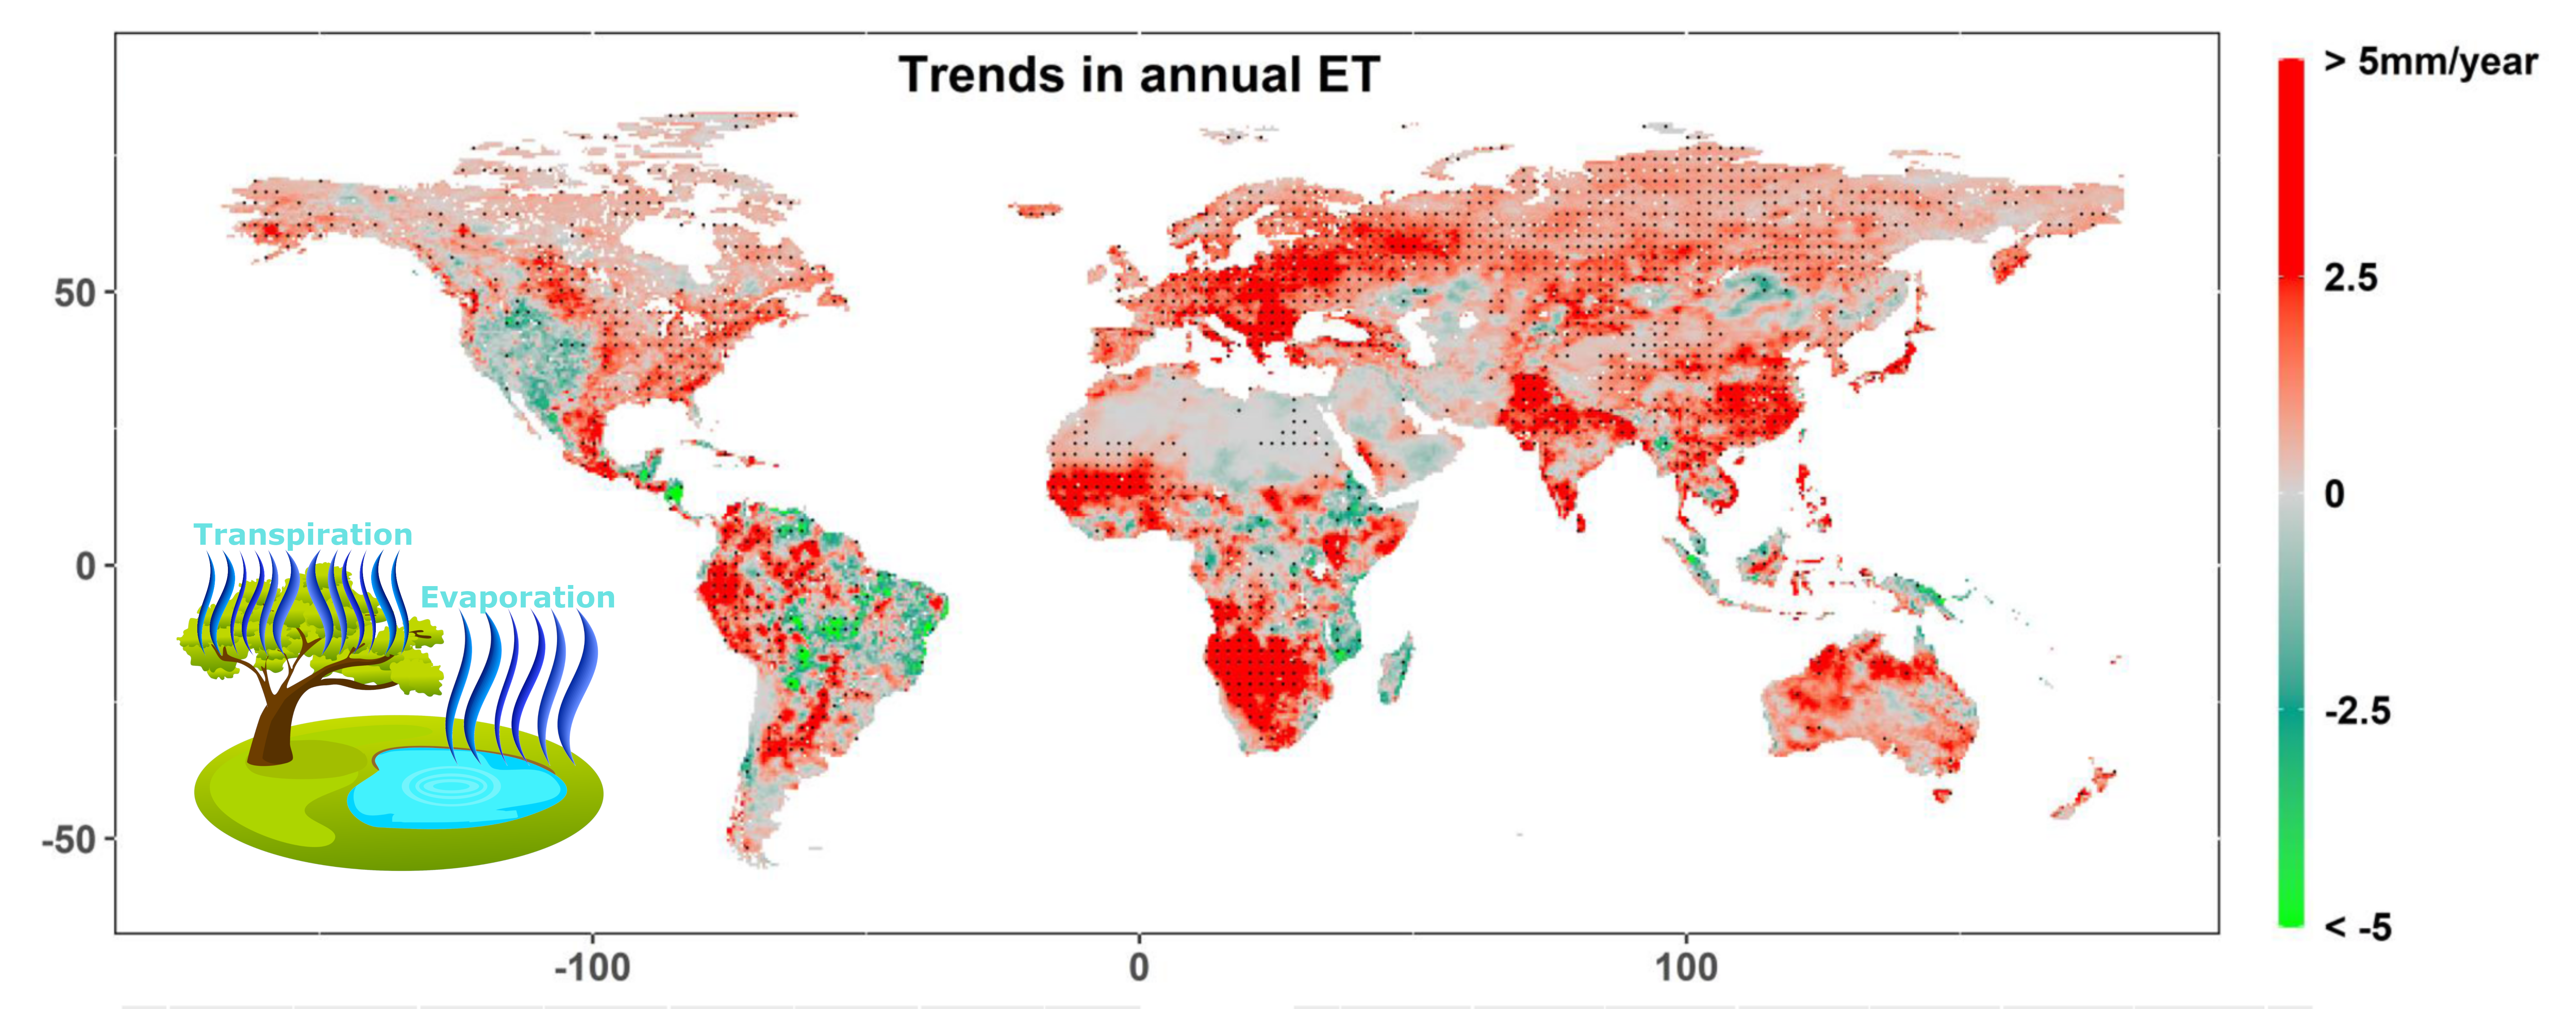
\includegraphics[width=\textwidth]{ET_Trends.png}}
	
	\vspace{1 em}
	
	So far, we have used ECOSTRESS to examine land surface temperatures. Today, we will explore a variable that \href{https://www.un.org/en/climatechange/science/climate-issues/water}{the United Nations considers to be at the center of the climate crisis: water.}

	\vspace{.5em}

	ECOSTRESS uses land surface temperatures to estimate an important water variable: evapotranspiration (ET). ET is the sum of all processes that return water from the land surface to the atmosphere and is comprised of two components:
	
\begin{itemize}
	\item 	Evaporation: process by which water is converted from a liquid on the earth's surface to vapor in the atmosphere.
 \item Transpiration: process by which water is lost from plants and returned to the atmosphere. The loss of water from plants is a consequence of the need for a permeable leaf surface that facilitates the uptake of $CO_2$ (e.g., through the stomata). Transpiration is a crucial component of the global terrestrial water cycle, as it returns around 60-70\% of water from the ground to the atmosphere. 

\end{itemize}

	The figure above, which was adapted from (\href{https://www.sciencedirect.com/science/article/pii/S016819232100349X?ref=pdf_download&fr=RR-2&rr=8052dedb59b02ea9}{Jianyu Liu et al. 2021}), shows that ET as a whole has been increasing for at least 80\% of the Earth between 1980 and 2017 as a result of anthropogenic change. 
	
\end{minipage}}

\section{Accessing ECOSTRESS Water Data through A$\rho\rho$EEARS}

\subsection{ECOSTRESS Data Product Levels}

ECOSTRESS has different levels of data products based on the amount of processing that is needed to create the data. Land surface temperature (LST) data is the primary observation from ECOSTRESS and forms the basis for the other products. LST is Level 2 (ECO2) after the calibration data in Level 1 (ECO1). Level 3 (ECO3) data is evapotranspiration, followed by products derived from evapotranspiration (ET), such as the evaporative stress index (ESI) and water use efficiency (WUE). Later tutorials will introduce ESI and WUE, while we focus here on ET. This table gives an overview of the ECOSTRESS data products: 

\vspace{.5em}

\centerline{\includegraphics[width=.75\textwidth]{ECOSTRESS_DataProducts.png}}

\vspace{.5em}

\subsection{Today's Study Location : California's Central Valley}

\begin{tcolorbox}[colback=yellow!5!white,colframe=IceCreamLeaf,title=\textbf{California's Central Valley}]
	\begin{multicols}{2}

	\centerline{\includegraphics[width=\columnwidth]{CentralValleyUSGS.png}}
	\columnbreak
		\begin{itemize}
			\item A vast agricultural region covering 20,000 square miles drained by the Sacramento and San Joaquin Rivers.
			\item Approximately 75\% of the irrigated land in California and 17\% of the irrigated land in the country is in the Central Valley.
			\item Using less than 1\% of U.S. farmland, the Central Valley produces $\frac{1}{4}$ of the food grown in the United States.
			\item About 20\% of the Nation's groundwater demand is supplied by pumping Central Valley aquifers, making it the second-most-pumped aquifer system in the U.S.
			\item As a result of climate change impacts in the Central Valley, there is a \href{https://www.energy.ca.gov/sites/default/files/2019-12/Water_CCCA4-EXT-2018-001_ada.pdf}{93\% likelihood of diminished groundwater delivery to millions of Californian households, businesses, and farms. There is also a 95\% probability of reduced drought resilience for crops}. 
		\end{itemize}
	\end{multicols}
\end{tcolorbox}

\begin{tcolorbox}[colback=yellow!5!white,colframe=IceCreamLeaf,title=\textbf{Hypotheses}]
	\begin{multicols}{2}

		\vspace*{.25em}

		\begin{itemize}
			\item Before we access the data, let's make some predictions about evapotranspiration:
			\item Given this map to the right with land surface temperatures observed by ECOSTRESS over the summer of 2022, where would you expect evapotranspiration to be the highest?
			\item Will hotter land surface temperatures correlate with higher rates of tranpsiration?
			\item To find out, we are going to download evapotranspiration data from ECOSTRESS, make a map of evapotranspiration, and compare that map with this land surface temperature map.
		\end{itemize}

		\columnbreak	

		\centerline{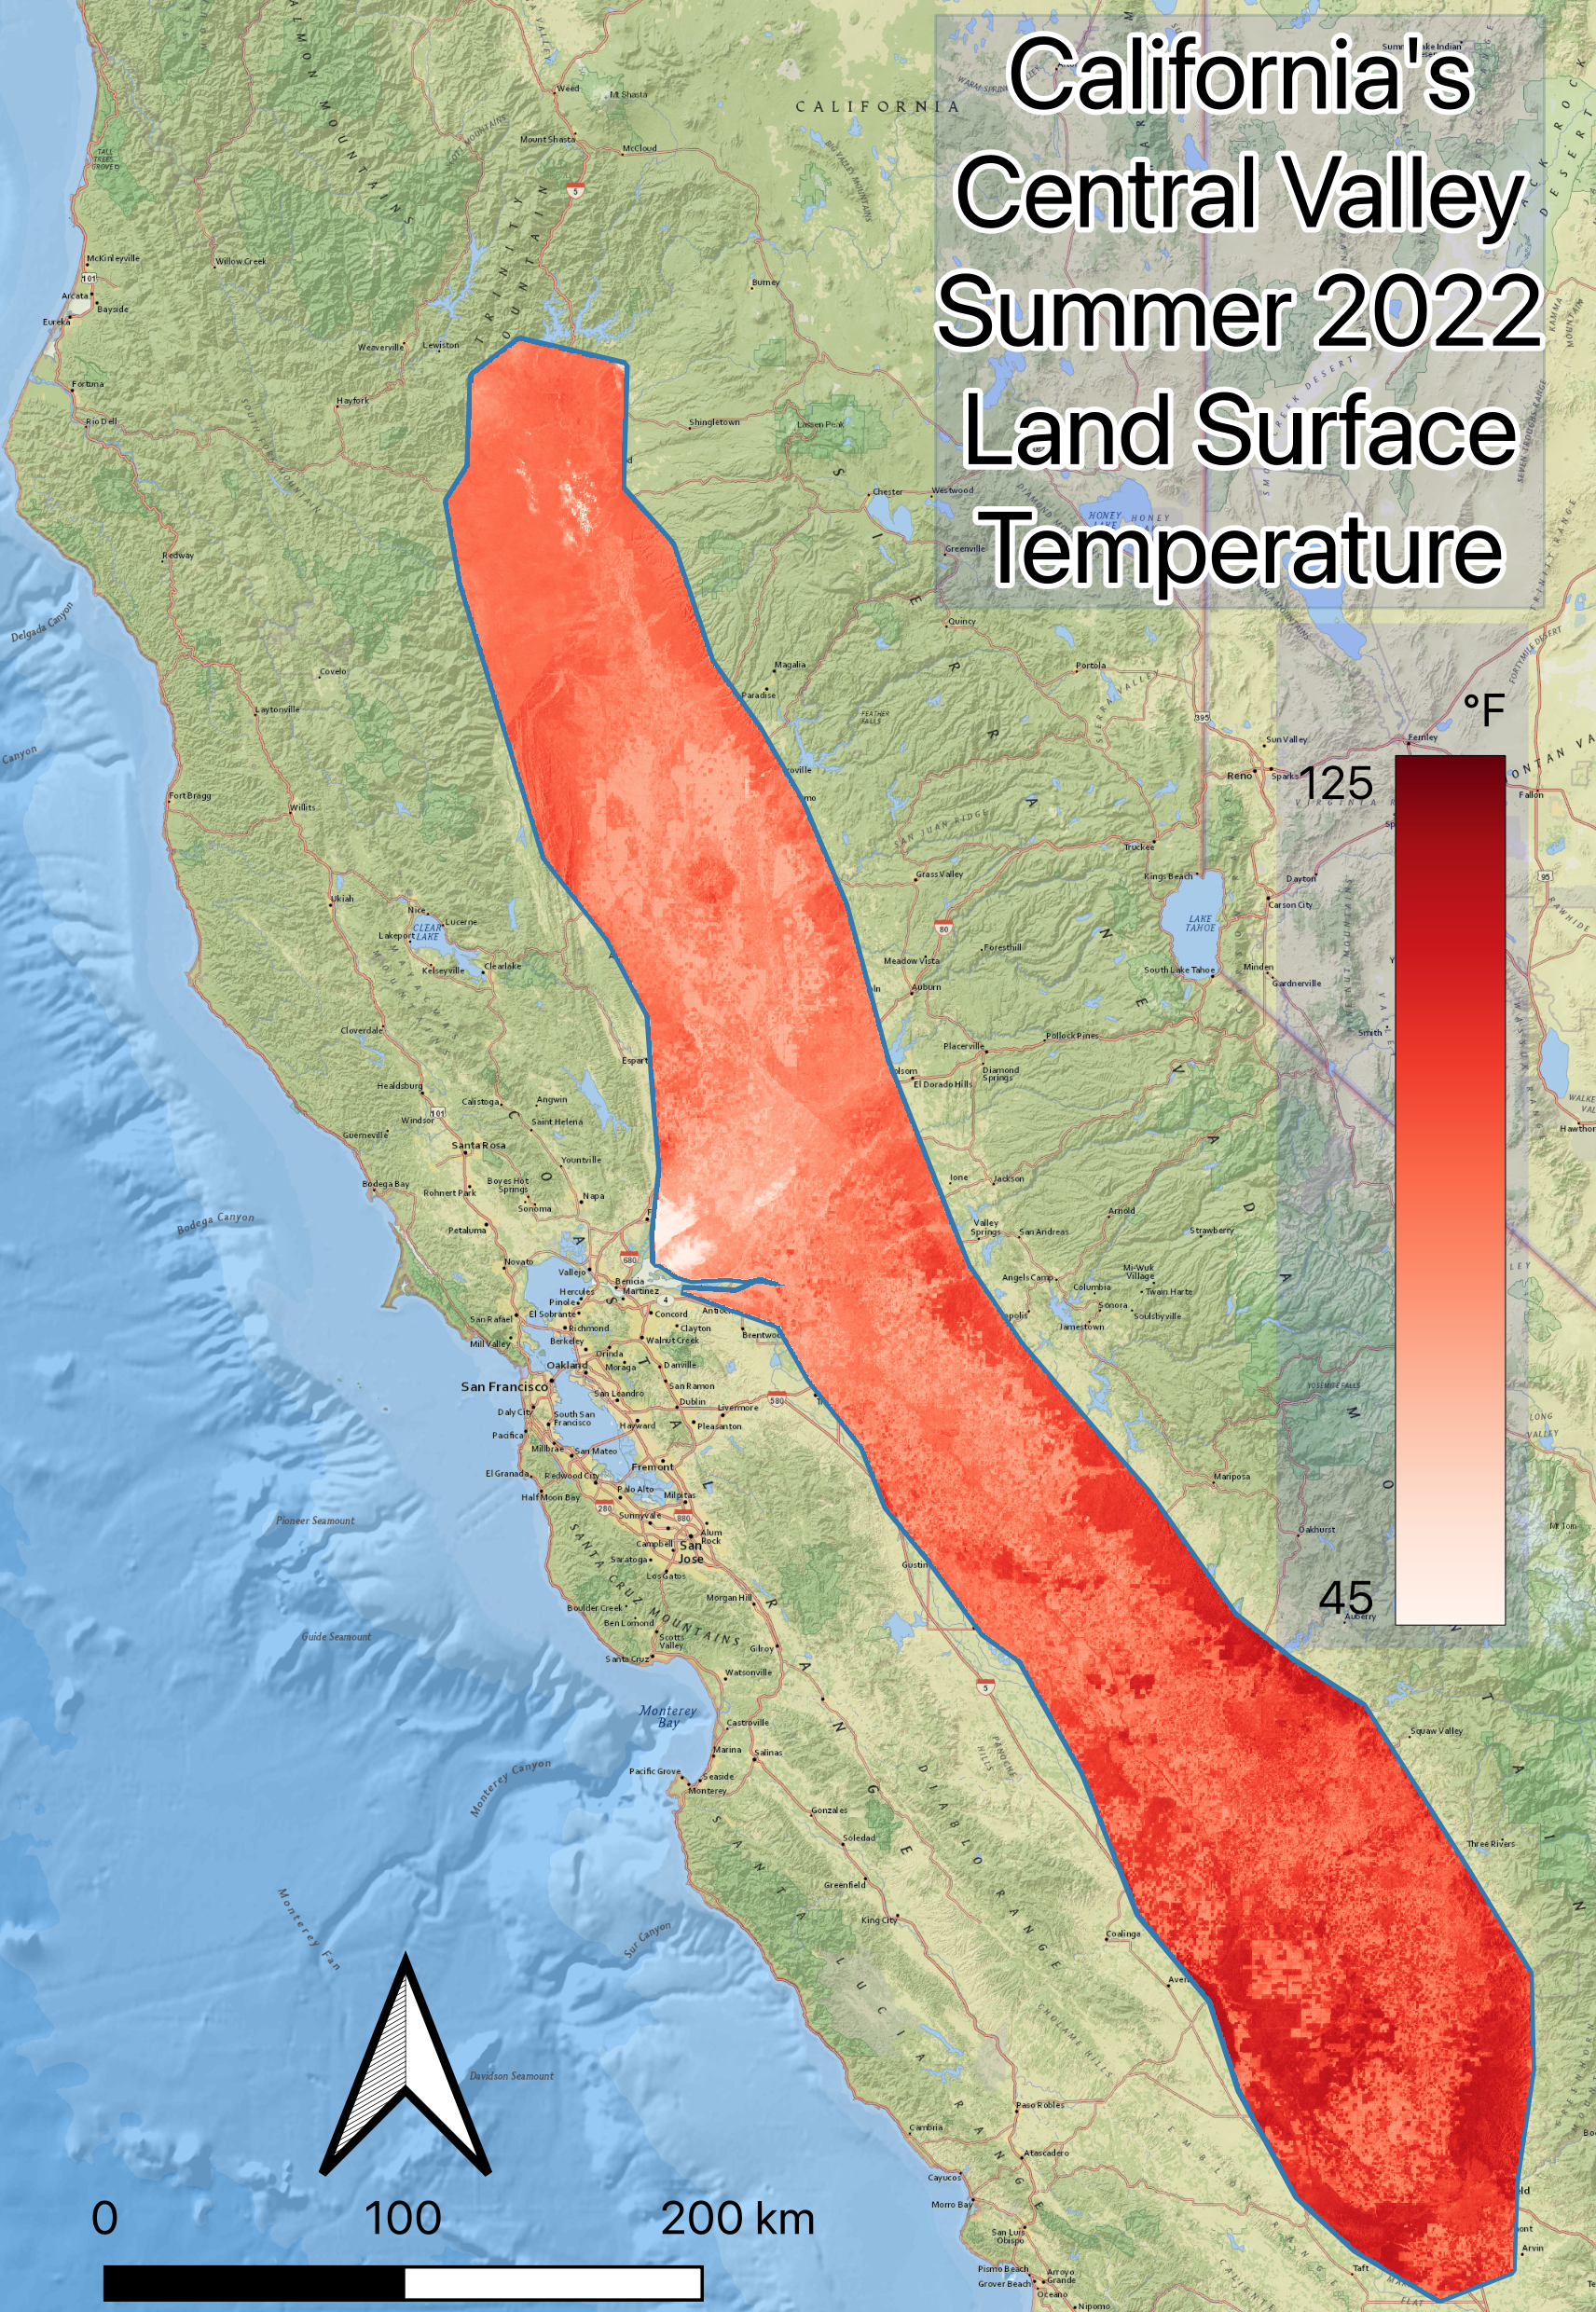
\includegraphics[width=\columnwidth]{CentralValleyLST.png}}
		
	\end{multicols}
\end{tcolorbox}

\subsection{Downloading Evapotranspiration from A$\rho\rho$EEARS}

The procedure for downloading ET data through the A$\rho\rho$EEARS interface is the same as the previous tutorials on land surface temperature.

1. Since we are focusing on California's Central Valley today, begin by downloading the file \href{https://jeremydforsythe.github.io/icecream-tutorials/Tutorial6_Evaportranspiration1/CaliforniaCentralValley.geojson}{CaliforniaCentralValley.geojson} and saving it somewhere you can remember. We recommend a folder containing all of the files for this tutorial. Depending on your web browser you may need to right click and select \textit{Save as}. Some web browsers may even display the contents of the GeoJSON file instead of prompting you to save it. If this happens you can select the \textit{File} dropdown menu and click on \textit{Save as}. 

\kulbox{\textbf{NOTE:} A .geojson file is an alternative to the shapefiles we have used to date. QGIS can import or export either format. An advantage of GeoJSON is that it is self-contained and does not need to be zipped before importing into A$\rho\rho$EEARS.}

2. Go to \href{https://appeears.earthdatacloud.nasa.gov/}{https://appeears.earthdatacloud.nasa.gov/} and login with your credentials. 

3. Use the \textit{Extract} dropdown menu to select \textit{Area}. Next select \textit{Start a New Request}. 

4. Enter a useful name for the request you are going to submit, maybe something like ``ET Central Valley Aug 6''. 

5. Drag and drop (or use the \textit{click here to select the file} link) to upload the GeoJSON file CaliforniaCentralValley.geojson. The map should be updated with a polygon encompassing California's Central Valley.

6. Update the \textit{Start} and \textit{End} Date Fields for our preselected date of interest: 08/06/2022 to 08/6/2022.

7. Under \textit{Select the layers to include in the sample} type the words ``ECOSTRESS'' and ``Evapotranspiration.'' Then scroll until you can click on \textit{ECOSTRESS Evapotranspiration PT-JPL}. From there, scroll until you see \textit{EVAPOTRANSPIRATION\_PT\_JPL\_ETdaily} and \textit{EVAPOTRANSPIRATION\_PT\_JPL\_ETinst} options. Click on the ``+'' signs to add those layers to your cart. Next, clear the selection of the current category using the small ``x'' to the right of the \textit{ECOSTRESS Evapotranspiration PT-JPL} box.

\centerline{\includegraphics[width=.6\textwidth]{ETRequest.png}}

\kulbox{\textbf{NOTE:} There are two models that can estimate evapotranspiration based on ECOSTRESS's measurement of  land surface temperature. One model, \href{https://ecostress.jpl.nasa.gov/downloads/atbd/ECOSTRESS_L3_ET_PT-JPL_ATBD_20180509.pdf}{``PT-JPL'',} is the most versatile and likely the best choice for most cases, including our experiment here today. The other option \href{https://ecostress.jpl.nasa.gov/downloads/userguides/ECOSTRESS_DisALEXI-JPL_L3_UserGuide_20210520_v2.pdf}{``DisALEXI-JPL''} has a different set of equations associated with it. If you are interested in evapotranspiration in agricultural settings, consider DisALEXI; otherwise, or if you are unsure, stay with PT-JPL.}

8. Under \textit{Output Options}, we want to use GeoTIFF (Geographic Tagged Image File Format; essentially an image file where the corresponding geographic information is embedded in the file) and \textit{Native Projection} for projection.

9. Click \textit{Submit} to complete the data request. At the top, you should see a green banner:

\vspace{.5em}

\centerline{\includegraphics[width=\textwidth]{RequestSuccess.png}}

\vspace{.5em}

10. Use the \textit{Explore} drop-down at the top to monitor the status of your request. It will likely go quickly, given that it is only one day's worth of data.

\vspace{.5em}

\centerline{\includegraphics[width=.75\textwidth]{ExploreRequest.png}}

\vspace{.5em}

\subsection{Downloading Evapotranspiration Component Data For The Next Tutorial}

11. In the meantime, we are going to create a request for the next tutorial, Tutorial 7, which continues to explore evapotranspiration by looking at the individual components. Setup a new request for data called ``ET Components,'' but this time we are going to select different variables. 

\vspace{.5em}

\centerline{\includegraphics[width=.6\textwidth]{ETcomponentRequest.png}}

\vspace{.5em}

12. Under the layer category ``\textit{ECOSTRESS Evaportanspiration PT-JPL}'' select ``\textit{EVAPORTRANSPIRATION\_PT\_JPL\_ETcanopy}'', ``\textit{EVAPOTRANSPIRATION\_PT\_JPL\_ETinterception}'', and ``\textit{EVAPOTRANSPIRATION\_PT\_JPL\_ETsoil}''.

13. Submit this request. We will return to it in Tutorial 7.

\vspace{.5em}

\centerline{\includegraphics[width=.6\textwidth]{ExploreComplete.png}}

\vspace{.5em}

\subsection{Data Check}

14. When your first request (``ET Central Valley Aug 6'') is complete, use the link on the \textit{Explore} page to access the details. Let's check out the data!

\vspace{.5em}

\centerline{\includegraphics[width=.6\textwidth]{ETinstDataCheck.png}}

\vspace{.5em}

15. Select the \textit{ECOSTRESS Evapotranspiration PT-JPL} layer.

16. Notice that there were different passes on the same day with very different values. Any ideas why? Checking the timestamps lets us know what is happening. The first three were at 02:00 in the morning when there is no sun and the plants are not transpiring.

17. To download the data from the daylight hours, select the small caret arrow in the gray box above and click on the \textit{Download} button.

18. Select the following filenames:

\begin{itemize}
	\item ECO3ETPTJPL.001\_EVAPOTRANSPIRATION\_PT\_JPL\_ETdaily\_doy2022218192026\_aid0001.tif
	\item ECO3ETPTJPL.001\_EVAPOTRANSPIRATION\_PT\_JPL\_ETdaily\_doy2022218191934\_aid0001.tif
	\item ECO3ETPTJPL.001\_EVAPOTRANSPIRATION\_PT\_JPL\_ETinst\_doy2022218192026\_aid0001.tif
	\item ECO3ETPTJPL.001\_EVAPOTRANSPIRATION\_PT\_JPL\_ETinst\_doy2022218191934\_aid0001.tif
\end{itemize}

\vspace{.5em}

\centerline{\includegraphics[width=.8\textwidth]{ETdownload.png}}

\vspace{.5em}

\kulbox{\textbf{NOTE:} ECOSTRESS estimates evapotranspiration at two time scales. The first, \textit{ET\_inst}, stands for instantaneous evapotranspiration and is calculated at the moment of the satellite pass. The other, \textit{ET\_daily}, is an estimate of the total evapotranspiration for the day of the satellite pass. We will examine this further later.}

19. Download the files using the \textit{Download} button that for some reason does not look much like a button on the top right corner of the screen. Save the files somewhere you can remember. 

\section{Visualizing ECOSTRESS Evapotranspiration Data in QGIS}

\subsection{Adding a Google Satellite Basemap}

20. Open QGIS and start a new project by selecting the \textit{Project} menu, then \textit{New}.

21. To add a basemap, find the \textit{HCMGIS} menu bar, select \textit{Basemap}, then pick your preferred map. For today's map, we will use \textit{Google Satellite}. Note that clicking on a basemap type automatically adds a new layer to your map, as seen in the layer browser window.

\subsection{Importing The NASA JPL Evapotranspiration Color ramp}

NASA has specifically designed a color palette to use with ECOSTRESS evapotranspiration data. \includegraphics[height= 1cm]{ETcolors.png} 

\vspace{.5em}

22. Download the color ramp file here: \href{https://jeremydforsythe.github.io/icecream-tutorials/Tutorial6_Evaportranspiration1/evapotranspirationJPLcolorramp.xml}{evapotranspirationJPLcolorramp.xml} and save it somewhere you can remember. Depending on your PDF viewer you may have to right-click and then hit \textit{Save As}.

23. From the \textit{Settings} top menu, select \textit{Style Manager}.

24. Select the ``Color Ramp'' tab.

25. Find and click on the \textit{Import/Export} button.

26. To the right of the \textit{File} input box click on the button with 3 dots (...). Select the evapotranspirationJPLcolorramp.xml file we just downloaded.

\centerline{\includegraphics[width=\textwidth]{ImportColorramp.png}} 

27. Click on the new ``evapotranspiration'' color ramp.

28. Click the \textit{Import} button.

29. Click the \textit{Close} button. We will use this color ramp in the next section of this tutorial.

\subsection{Add in evapotranspiration layer(s)}

\centerline{\includegraphics[width=\textwidth]{ETmapping.png}}

30. Use the \textit{browser} window to find the folder where you saved the two instantaneous evapotranspiration .tif files: 
\begin{itemize}
	\item ECO3ETPTJPL.001\_EVAPOTRANSPIRATION\_PT\_JPL\_ETinst\_doy2022218192026\_aid0001.tif
	\item ECO3ETPTJPL.001\_EVAPOTRANSPIRATION\_PT\_JPL\_ETinst\_doy2022218191934\_aid0001.tif
\end{itemize}
Double-click each file to add them to your map. Again, notice that they are now also listed in the \textit{Layers} window.

31. Now you have ECOSTRESS evapotranspiration data on your map. But wait, if you recall from our Death Valley Land Surface Temperature maps, QGIS does not know the type of data you are using and has defaulted to displaying the information in grayscale. For each of the evapotranspiration layers, right-click on the layer name in the \textit{Layers} window and select \textit{Layer Properties}. 

32. On the menu bar to the left, select \textit{Symbology} and change \textit{Render type} to Singleband pseudocolor. 

33. QGIS has automatically determined the minimum and maximum values from the datafiles; however, we have two files, so we need to match them. Specify 0 as the minimum and 715 as the maximum. Click apply.

34. To access the fancy new color ramp we just downloaded click on the color ramp button.

35. Select \textit{All Color Ramps}.

36. Select our new \textit{Evapotranspiration} color ramp. 

37. Finally, add the border from CaliforniaCentralValley.geojson by double clicking on it in the \textit{Browser} window. Right-click (ctrl-click on Mac) on the layer in the \textit{Layers} window and change the symbology to \textit{outline red}. 

\kulbox{\textbf{NOTE:} There was not full data coverage for the entire Central Valley available, that is why the northern and southern most part of the outline does not have any color overlayed. This sometimes happens because of the orbit of the space station. If we were interested in filling in the gaps, we would look for passes plus or minus one week around the same time of day and form a composite.}

\section{Add Map Elements}

34. Following the procedure described in \href{https://jeremydforsythe.github.io/icecream-tutorials/Tutorial5_AddingElementsToMaps/Tutorial5_AddingElementsToMaps.pdf}{Tutorial \#5 : Adding Elements To Maps}, make a professional map complete with scalebars, labels, a legend, titles, and a North arrow. Include a basemap showcasing the study area (California's Central Valley) and two inset maps. The one that we just created now for the instantaneous evapotranspiration data and one using the daily scale (ETdaily) GeoTIFF files we downloaded. This map will be your map of the week assignment.

\begin{tcolorbox}[colback=yellow!5!white,colframe=IceCreamOrbit,title= \vspace{.2em} \Large Map of the Week Assignments]
	\addcontentsline{toc}{section}{Map of the Week Assignments}
	\large
	\begin{enumerate}
		\item Make an evapotranspiration map for California's central valley with two insets, one for the instantaneous evapotranspiration data and one for the daily evapotranspiration data we downloaded in the tutorial for August 6, 2022 (day of the year 218). The map should be complete with scalebars(s), north arrow(s), legend(s), title(s), and label(s). 
        \item Provide a 1-2 paragraph description of your map that includes your hypotheses about how land surface temperature would influence evapotranspiration. Does your map support your hypotheses? How did instantaneous and daily data differ? How is it possible that daily evapotranspiration is less than instantaneous?
	\end{enumerate}
	Submit these assignments via Canvas before Monday's class.
\end{tcolorbox}

\begin{tcolorbox}[colback=yellow!5!white,title=\textbf{Datafiles}]
	\addcontentsline{toc}{section}{Datafiles}
	\large
	In case you encountered any issues with the A$\rho\rho$EEARS database, here are copies of the ECOSTRESS GeoTIFF files for the Central Valley of California. $ET_{inst}$:
	\begin{enumerate}
		\item \href{https://jeremydforsythe.github.io/icecream-tutorials/Tutorial6_Evaportranspiration1/ECO3ETPTJPL.001_EVAPOTRANSPIRATION_PT_JPL_ETinst_doy2022218192026_aid0001.tif}{\small ECO3ETPTJPL.001\_EVAPOTRANSPIRATION\_PT\_JPL\_ETinst\_doy2022218192026\_aid0001.tif}
		\item \href{https://jeremydforsythe.github.io/icecream-tutorials/Tutorial6_Evaportranspiration1/ECO3ETPTJPL.001_EVAPOTRANSPIRATION_PT_JPL_ETinst_doy2022218191934_aid0001.tif}{\small ECO3ETPTJPL.001\_EVAPOTRANSPIRATION\_PT\_JPL\_ETinst\_doy2022218191934\_aid0001.tif}
	\end{enumerate}
	And $ET_{daily}$:
	\begin{enumerate}
		\item \href{https://jeremydforsythe.github.io/icecream-tutorials/Tutorial6_Evaportranspiration1/ECO3ETPTJPL.001_EVAPOTRANSPIRATION_PT_JPL_ETdaily_doy2022218192026_aid0001.tif}{\small ECO3ETPTJPL.001\_EVAPOTRANSPIRATION\_PT\_JPL\_ETdaily\_doy2022218192026\_aid0001.tif}
		\item \href{https://jeremydforsythe.github.io/icecream-tutorials/Tutorial6_Evaportranspiration1/ECO3ETPTJPL.001_EVAPOTRANSPIRATION_PT_JPL_ETdaily_doy2022218191934_aid0001.tif
}{\small ECO3ETPTJPL.001\_EVAPOTRANSPIRATION\_PT\_JPL\_ETdaily\_doy2022218191934\_aid0001.tif}
	\end{enumerate}
\end{tcolorbox}

%%%%%%%%%%%%%%%%%%%%%%%%%%%%%%%%%%%%%%%%%%%%%%%%%%%%%%%%%%%%%%%%%%%%%%%%%%%%%%%%%%% End of Document
%\vfill

\hrule

\vspace{1em}

\small \textbf{Recommended Citation:} Forsythe, J.D., G.R. Goldsmith, and J.B. Fisher. 2023. Observing Earth from Above Tutorials. Chapman University. \url{https://jeremydforsythe.github.io/icecream-tutorials/}

\vspace{1em}

This work is supported by funding from NASA ECOSTRESS Mission Grant \#80NSSC23K0309 (I.C.E. C.R.E.A.M.: Integrating Communication of ECOSTRESS Into Community Research, Education, Applications, and Media).

\end{document}
